%---------------
% Question 1
%---------------

\begin{question}{1}
\end{question}
\textbf{Example 2.2-1} describes a process in which a performance measure and
associated weights can be determined for controlling the attitude, $\theta(t)$,
of a manned spacecraft using gas expulsion system, shown in Figure \ref{fig:spacecraft_acs}.
The objective of the control system is to maintain the attitude of the
spacecraft at $\theta(t) = 0$ and to do with with small accelerations.

\begin{figure}[h]
    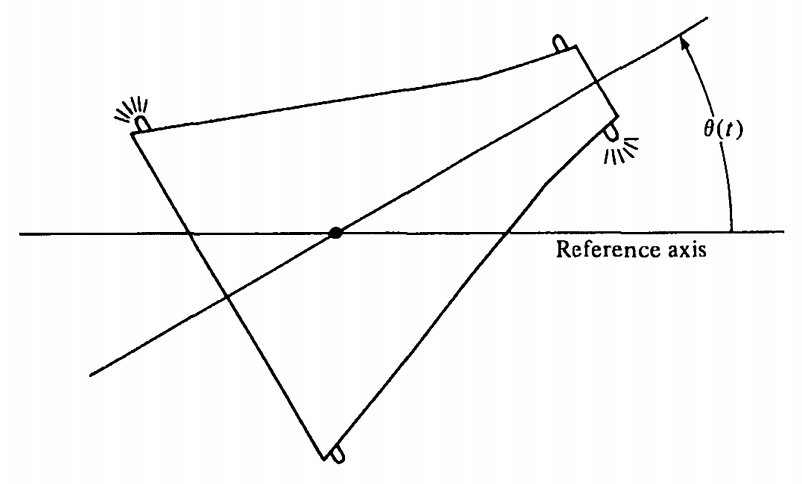
\includegraphics[scale=0.35]{spacecraft_acs}
    \centering
    \caption{Attitude control of a spacecraft \cite{kirkdover}}
    \label{fig:spacecraft_acs}
\end{figure}

The dynamics of the system are given by the differential equation given in
Equation \ref{eq:spacecraft_acs}. 
\begin{equation}
    I \ddot{\theta}(t) = \lambda(t) \label{eq:spacecraft_acs}
\end{equation}

\noindent where $I$ is angular moment of inertia and $\lambda(t)$ is the
torque produced by the gas jets. The state space equations are

\begin{align}
    \dot{x_1}(t) &= x_2 (t) \label{eq:sc_ssr_s1} \\
    \dot{x_2}(t) &= u (t) \label{eq:sc_ssr_x2}
\end{align}

\noindent where $u(t) = \dfrac{1}{I} \lambda(t)$. The performance measure is 
given in Equation \ref{eq:spacecraft_pf} below

\begin{equation}
    J = \int_{0}^{\infty} [q_{11} x_1^2(t) + q_{22} x_2^2(t) + R u^2 (t)] \, dt
    \label{eq:spacecraft_pf}
\end{equation}



